\documentclass[11pt, american, draft]{PhdThesis}

\usepackage[american]{babel}
\usepackage[final]{graphicx}

\usepackage[T1]{fontenc}
\usepackage{enumitem}
\usepackage{forest}
\usepackage{url}
\usepackage{float}

\forestset{
  default preamble = {
    for tree = {draw, ellipse}
  }
}

\author{Matteo Morena}
\email{morena.matteo@gmail.com}
\supervisor{Marco Comini}
\title{Implementation of an interpreter with graphical interface of a simple imperative language}
\date{2021--2022}

\begin{document}
  \pagestyle{empty}
  \maketitle

  % \begin{dedication}
  %   TBD
  % \end{dedication}

  % \begin{abstract}
  %   TBD
  % \end{abstract}

  % \begin{acknowledgments}
  %   TBD
  % \end{acknowledgments}

  \frontmatter
  \partstyle{serifbig}
  \chaptertitlestyle{serifbig}
  \pagestyle{serif}
  \tableofcontents
  % \listoffigures
  % \listoftables

  % \introduction
  % TBD

  % \section*{an intro section}
  % TBD

  \mainmatter

  % \chapter{Preliminaries}
  % TBD

  % \section{a preliminaries section}
  % TBD

  \chapter{Parsing}

  The first phase of any compiler or interpreter is called \emph{parsing}. The purpose of this
  phase is to analyze an input string and determine if it conforms to some set of rules; if it
  does, a logical representation of the input is constructed.

  \section{Languages and grammars}

  Consider a parser for arithmetic expressions. The input of the parser is any sequence of
  characters. Invalid strings like \verb$(1 +)$ and \verb$(3 * * 4)$ get rejected. Valid strings
  like \verb$(2 * (3 + 4))$ get accepted.

  The \emph{language} accepted by a parser is the set of all possible inputs which the parser may
  accept. The set of rules to which the input has to conform to is called the \emph{grammar} of the
  language.

  As an example, we could define the grammar for arithmetic expressions as follows:

  \begin{itemize}[noitemsep,topsep=0pt]
    \item A sequence of characters representing a number is a \emph{literal expression}.

    \item If $x$ is an expression, then \verb$($, followed by $x$, followed by \verb$)$ is a
          \emph{parenthesized expression}.

    \item If $x$ is a literal or parenthesized expression, then $x$, preceded by a unary operator,
          is a \emph{unary expression}. An unary operator is one of the following characters:
          \verb$+$, \verb$-$.

    \item If $x$ and $y$ are unary or parenthesized expressions, then $x$, followed by a
          multiplicative operator, followed by $y$, is a \emph{multiplicative expression}. A
          multiplicative operator is one of the following characters: \verb$*$, \verb$/$.

    \item If $x$ and $y$ are multiplicative or parenthesized expressions, then $x$, followed by an
          additive operator, followed by $y$, is an \emph{additive expression}. An additive operator
          is one of the following characters: \verb$+$, \verb$-$.
  \end{itemize}

  According to such rules, the string \verb$(2 * (3 + 4))$ is a valid arithmetic expression. By
  definition:

  \begin{itemize}[noitemsep,topsep=0pt]
    \item \verb$2$, \verb$3$ and \verb$4$ are literals;
    \item \verb$3 + 4$ is an additive expression;
    \item \verb$(3 + 4)$ is a parenthesized expression;
    \item \verb$2 * (3 + 4)$ is a multiplicative expression;
    \item \verb$(2 * (3 + 4))$ is an expression.
  \end{itemize}

  \section{Syntax trees}

  A \emph{syntax tree} is the representation of a string accepted by the parser; this data
  structure stores the syntactic structure of the input.

  A syntax tree may retain all information necessary to reconstruct the input; in this case, it is
  called a \emph{concrete} syntax tree. If some information about the source is discarded
  (comments, for example), it is called an \emph{abstract} syntax tree.

  Consider the language of arithmetic expressions: we can think of at least two possible syntax
  trees for the string \verb$(2 + 3 * (4 + 5))$, depending on how much information has been kept.
  When information is thrown away, the semantic meaning stays the same: for instance, details about
  parenthesization can be discarded if the resulting syntax tree still represents the same order of
  operations.

  \begin{figure}[H]
    \centering

    \begin{ttfamily}
      \begin{forest}[+ [2] [* [3] [+ [4] [5]]]]\end{forest}
      \begin{forest}[( ) [+ [2] [* [3] [( ) [+ [4] [5]]]]]]\end{forest}
    \end{ttfamily}

    \caption{Two semantically equivalent syntax trees for \mbox{\texttt{(2 + 3 * (4 + 5))}}}
  \end{figure}

  As we'll see later, the parser for Devin uses a single tree representation which retains enough
  information for syntax highlighting, but also discards whitespace. For our purposes, the
  distinction between abstract and concrete syntax tree isn't necessary: for this reason, from now
  on I'll just use the term \emph{syntax tree}.

  \section{Parser combinators}

  There are many ways to recognize some input and generate an associated syntax tree. There has been
  much academic research, and it is trivial to find so-called \emph{parser generators}: these are
  tools which, given a grammar, automatically generate code for parsing the language in question.
  Such tools build upon well-known algorithms, such as LL, LR, LALR, just to throw a few names
  around. These tools are great and very performant; however, they're kind of magical.

  In this section, we'll see how there's no fundamental need for any generators; although such tools
  are handy, it isn't actually that difficult to write a parser from scratch, using a technique
  called \emph{recursive descent parsing}. Recursive descent parsers are used by the GCC compiler
  and the V8 JavaScript engines, for example\cite{nystrom}.

  Recursive descent is a method of constructing a parser using a collection of recursive functions.
  The simplest functions parse the atoms (or \emph{tokens}) of the target language; examples of such
  functions are parsers for numbers and identifiers. By gluing together simpler functions, more
  complex parsers can be created: for example, a parser for two-dimensional coordinates
  \mbox{\texttt{($x$, $y$)}} can be built by using the parsers for open-parenthesis, number, comma,
  number, and close-parenthesis respectively. Finally, parsers can be combined recursively: a parser
  $P$ could depend on a parser $Q$, which in turn depends on $P$. Consider any language supporting
  \verb$while$ statements: the body of the \verb$while$ is yet another statement, which in turn
  could be a \verb$while$ statement.

  Recursive descent can be implemented in any imperative language; of course, a similar technique
  can be applied to functional programming as well. The functional approach lends itself perfectly
  for this kind of task; in particular, higher order functions abstract the boilerplate necessary to
  glue together different parsing functions. These higher order functions are called \emph{parser
  combinators}, as they combine simpler parsers into more complex ones.

  The general interface employed by parser combinators is that of a function which takes some input
  string; the function returns either an error or some result together with the remaining input. For
  instance, applying the function parsing an integer on the input string \verb$21*2$ yields the
  pair \mbox{$\left(21, \texttt{*2}\right)$}.

  Some common parser combinators are:

  \begin{itemize}[noitemsep,topsep=0pt]
    \item The \emph{sequence combinator}. Informally, this combinator runs two parsers in succession
          and combines their results.

          Let $P$ and $Q$ be two parsers. The sequence combinator runs $P$; if it succeeds, then $Q$
          is run on the remaining input. If $Q$ also succeeds, the combinator succeeds with the
          combined results of $P$ and $Q$. If $P$ or $Q$ fail, then the combinator also fails.

    \item The \emph{alternative combinator}. Informally, this combinator implements choice.

          Let $P$ and $Q$ be two parsers. The alternative combinator runs $P$ and $Q$ on the same
          input. If $P$ succeeds, the combinator succeeds with the same result as $P$ did; if $Q$
          succeeds, the combinator succeeds with the same result as $Q$ did. If both $P$ and $Q$
          fail, then the combinator also fails.

    \item The \emph{option combinator}. Informally, this combinator runs a parser zero or one time.

          Let $P$ be a parser. The option combinator tries to run $P$. If $P$ succeeds, the
          combinator succeeds with the same result as $P$ did. If $P$ fails, the combinator succeeds
          with an empty result.

    \item The \emph{repetition combinator}. Informally, this combinator runs a parser many times.

          Let $P$ be a parser. The repetition combinator tries to run $P$ as many times as possible,
          until $P$ fails. Each time $P$ succeeds, the remaining input is fed back into the next
          application of $P$ itself. This combinator succeeds with the accumulated results of all
          successful runs.

    \item The \emph{bind combinator}. Informally, this combinator allows one parser to depend on the
          result of another parser. As we will see, this is the most powerful combinator of them
          all. All others could be expressed in terms of the bind combinator.

          Let $P$ be a parser and $f$ a one-parameter function yielding
          another parser. The bind combinator tries to run $P$; if it succeeds, it applies $f$ on
          the result of $P$, running the resulting parser on the remaining input. If $P$ fails, this
          combinator also fails.
  \end{itemize}

  \chapter{Tree traversal}

  Once a syntax tree has been constructed by the parser, the tree can be traversed in a multitude of
  ways. In general, syntax trees can not only represent the structure of a programming languages,
  but also the structure of markup languages or other kinds of structured languages. For the
  purposes of this thesis, I'll discuss the processing of programming languages only.

  It is important to note the grammar of a language only describes its \emph{syntax}: on its own,
  it only defines which inputs strings are valid, and which are not. Similarly, a parser only
  transforms syntactically valid input strings into trees: it is the role of other components to
  give \emph{semantic meaning} to such trees.

  \begin{itemize}[noitemsep,topsep=0pt]
    \item An \emph{evaluator} would associate the nodes of a syntax tree with actions to execute.
          Examples of such actions are performing arithmetic calculations, conditionally executing
          other nodes, and assigning or retrieving values from variables.

    \item A \emph{compiler} would translate a syntax tree into some other form. For instance, the
          GCC compiler produces object files from valid C syntax; in turn, object files can be
          parsed by the system's linker, which translates a collection of such files into a runnable
          executable.

    \item On languages where the semantics involve static types, a \emph{type checker} would verify
          that no type errors would be produced by evaluation or compilation. In such systems, the
          type checker coexists with an evaluator or compiler (or both); it is fundamental that all
          components obey to the same semantics. Often, the evaluator or compiler depends on some
          additional information provided by the type checker: this won't be the case for Devin.

    \item Similarly to type checking, a \emph{linter} would analyze the syntax tree as well.
          Contrary to the type checking, the linter may not depend on static types (if any);
          furthermore, successful compilation or execution doesn't depend on linting. Rather, the
          linter suggests how the original source could be improved. Like with the type checker, all
          components must obey to the same semantics.

    \item A \emph{syntax highlighter} would use the information stored in a syntax tree to perform
          syntax highlighting. Such a syntax tree would be rather concrete, as each node would be
          associated with a position in the parser's input string.
  \end{itemize}

  \section{Evaluation}

  \section{Type checking}

  \section{Syntax highlighting}

  \section{The monadic interface}

  \chapter{A first look at Devin}

  In this thesis, I'll discuss the implementation of a simple imperative programming language which
  I decided to call Devin. The name Devin is an homage to Duino, the city I'm currently living in;
  its slovenian name is, in fact, Devin.

  Alongside Devin, I developed a graphical text editor for the language. The editor features syntax
  highlighting, error reporting, and a simple visual debugger.

  \begin{figure}[H]
    \centering
    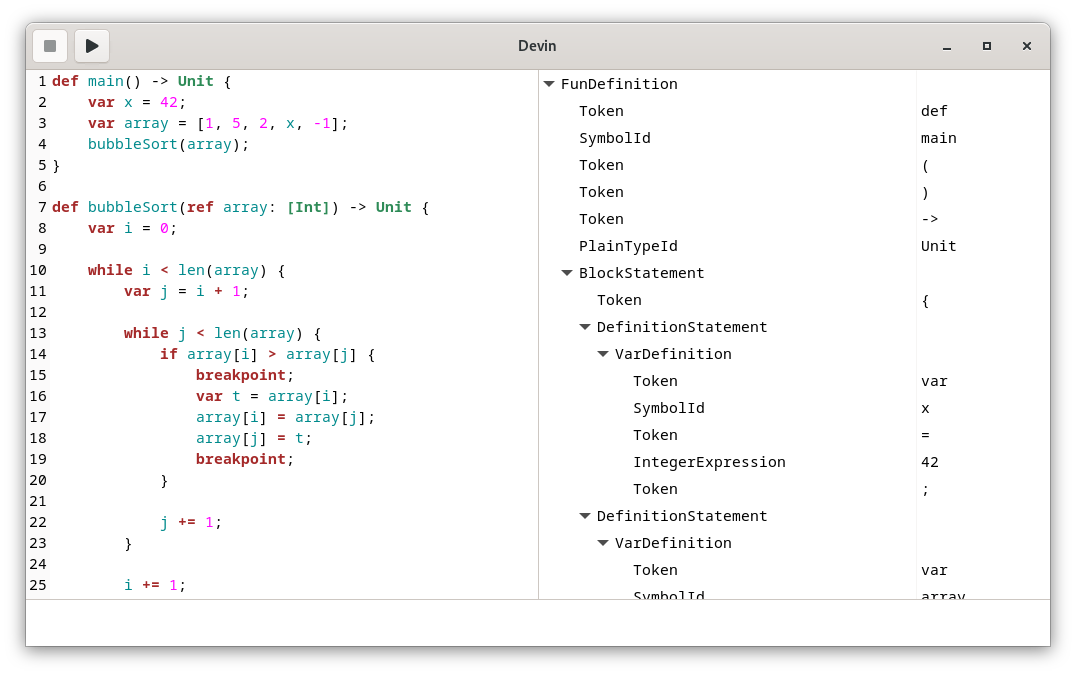
\includegraphics[width=0.9\linewidth]{2.png}
    \caption{The graphical editor associated with Devin}
    \label{ex1}
  \end{figure}

  \section{Language features}

  Devin is an imperative procedural programming language with lexical variable scoping and support
  for recursive function definitions. Syntactically, it is very similar to any C descendant; it
  supports \verb$while$ loops, \verb$do-while$ loops and variable assignment. Two significant
  differences from C-like languages are the syntax required to specify parameter types and the lack
  of \verb$for$ loops. A more complex program example can be seen in figure \ref{ex1}.

  \subsection{Built-in data types and expressions}

  Devin supports the following data types:

  \begin{itemize}[noitemsep,topsep=0pt]
    \item \verb$Int$: 64-bit integers like \verb$11$, \verb$+12$ and \verb$-42$;

    \item \verb$Float$: double-precision floating-point numbers like \verb$34.12$, \verb$+11.0$ and
          \verb$-2.56$;

    \item \verb$Bool$: the boolean values \verb$true$ and \verb$false$.
  \end{itemize}

  Like functional programming languages, Devin has a \emph{unit type} \verb$Unit$; it is inhabited
  by one value only: \verb$unit$. Unit types can be used is in lieu of void types: when a
  procedure has side effects only, it marked as returning \verb$Unit$. Unit types simplify language
  development, as they remove the distinction between procedures which return some value
  and those who don't.

  The evaluation strategy of Devin is strict; function arguments are passed by value or by
  reference, depending on the signature of the callee. In both cases, the syntax for function
  application is the same.

  Integers and floating-point numbers support the following set of operations:

  \begin{itemize}[noitemsep,topsep=0pt]
    \item \emph{Unary negation}: \mbox{\texttt{-$x$}};

    \item \emph{Identity}: \mbox{\texttt{+$x$}};

    \item \emph{Addition}: \mbox{\texttt{$x$ + $y$}};

    \item \emph{Subtraction}: \mbox{\texttt{$x$ - $y$}};

    \item \emph{Multiplication}: \mbox{\texttt{$x$ * $y$}};

    \item \emph{Division}: \mbox{\texttt{$x$ / $y$}}. If $x$ and $y$ are integers, the result is
          \mbox{$\lfloor\frac{x}{y}\rfloor$};

    \item \emph{Modulo}: \mbox{\texttt{$x$ \% $y$}}. It is only defined if $x$ and $y$ are both
          integers; it is \mbox{$x - y \lfloor\frac{x}{y}\rfloor$};

    \item \emph{Comparison}: \mbox{\texttt{$x$ < $y$}}, \mbox{\texttt{$x$ <= $y$}},
          \mbox{\texttt{$x$ > $y$}}, \mbox{\texttt{$x$ >= $y$}}.
  \end{itemize}

  Booleans support the following set of operations:

  \begin{itemize}[noitemsep,topsep=0pt]
    \item \emph{Unary negation}: \mbox{\texttt{not $x$}};
    \item \emph{Logical conjunction}: \mbox{\texttt{$x$ and $y$}};
    \item \emph{Logical disjunction}: \mbox{\texttt{$x$ or $y$}};
    \item \emph{Exclusive disjunction}: \mbox{\texttt{$x$ xor $y$}}.
  \end{itemize}

  Comparison in the form of \mbox{\texttt{$x$ == $y$}} and \mbox{\texttt{$x$ != $y$}} is supported
  between operands any type.
  
  Finally, all values can be reassigned with the \verb$=$ operator. Devin supports the following assignment
  shorthands:

  \begin{itemize}[noitemsep,topsep=0pt]
    \item \mbox{\texttt{$x$ += $y$}}, which is the same as \mbox{\texttt{$x$ = $x$ + $y$}};
    \item \mbox{\texttt{$x$ -= $y$}}, which is the same as \mbox{\texttt{$x$ = $x$ - $y$}};
    \item \mbox{\texttt{$x$ *= $y$}}, which is the same as \mbox{\texttt{$x$ = $x$ * $y$}};
    \item \mbox{\texttt{$x$ /= $y$}}, which is the same as \mbox{\texttt{$x$ = $x$ / $y$}};
    \item \mbox{\texttt{$x$ \%= $y$}}, which is the same as \mbox{\texttt{$x$ = $x$ \% $y$}}.
  \end{itemize}

  TODO--

  with the \texttt{ref} keyword, they can be passed by reference instead. In any case, argument
  evaluation always happens from left to right.

  \begin{figure}[H]
    \center

    \begin{verbatim}
def sum1(a: Int, b: Int) -> Int
    return a + b;

def sum2(a: Int, b: Int, ref into: Int) -> Unit
    into = a + b;
    \end{verbatim}

    \caption{Two different ways of writing a procedure summing up two numbers}
    \label{ex2}
  \end{figure}

  A peculiar feature of Devin is that of \emph{optional types}. With optional types, the semantic of
  the language doesn't depend on the type system; instead, as Gilad Bracha proposed\cite{bracha}, a
  type system can be plugged into the language at will. A notable example of an optionally typed
  language is Python. In Devin, the type system is not pluggable per se, however it is independent
  of the evaluator; thus, it but could be easily replaced by modifying its source code.

  Type annotations can be omitted from Devin programs, as shown in figure \ref{ex3}. Type checking
  is not performed on terms where type annotations are missing. Effectively, this makes Devin
  statically typed only if \emph{all} terms are annotated; otherwise, it is dynamically typed to
  varying degrees.

  \begin{figure}[H]
    \center

    \begin{verbatim}
def sum1(a, b)
    return a + b;

def sum2(a, b, ref into)
    into = a + b;
    \end{verbatim}

    \caption{Two procedures summing up two numbers, written without type annotations}
    \label{ex3}
  \end{figure}

  Another feature of Devin is that of type inference for variable declarations. Unlike in C, the
  type of local variables has not to be specified.

  \begin{figure}[H]
    \center

    \begin{verbatim}
def swap(ref a: Int, ref b: Int) -> Unit {
    var t = a;
    a = b;
    b = t;
}
    \end{verbatim}

    \label{ex4}
    \caption{TODO}
  \end{figure}

  \section{Editor features}

  \begin{figure}[H]
    \center
    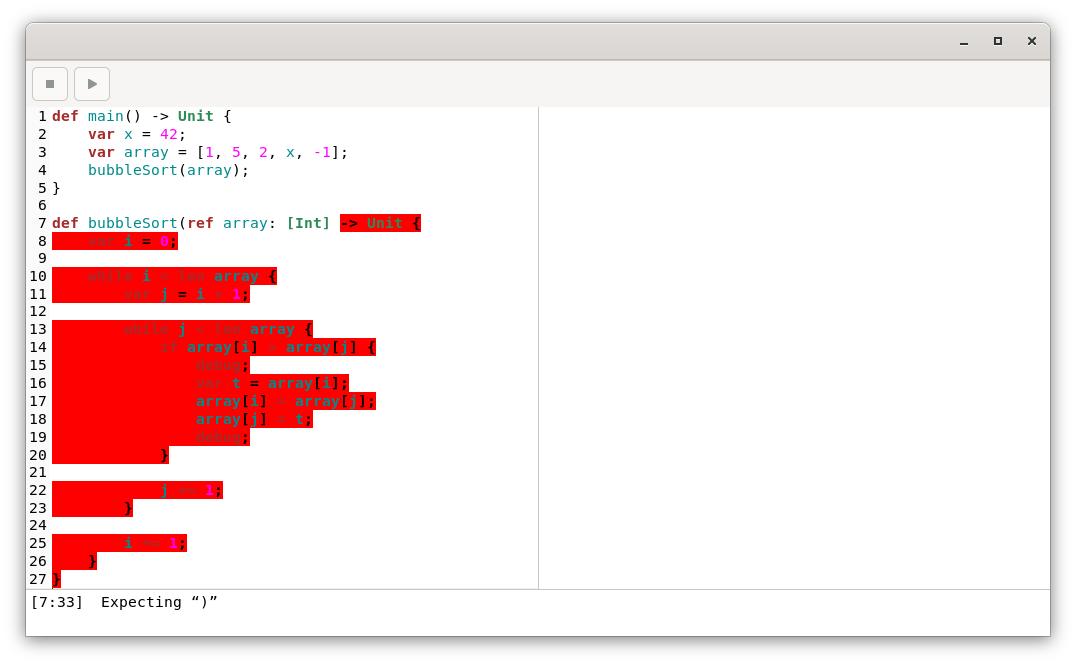
\includegraphics[width=0.9\linewidth]{3.png}
    \caption{Syntax error reporting and highlighting}
    \label{ex5}
  \end{figure}

  \begin{figure}[H]
    \center
    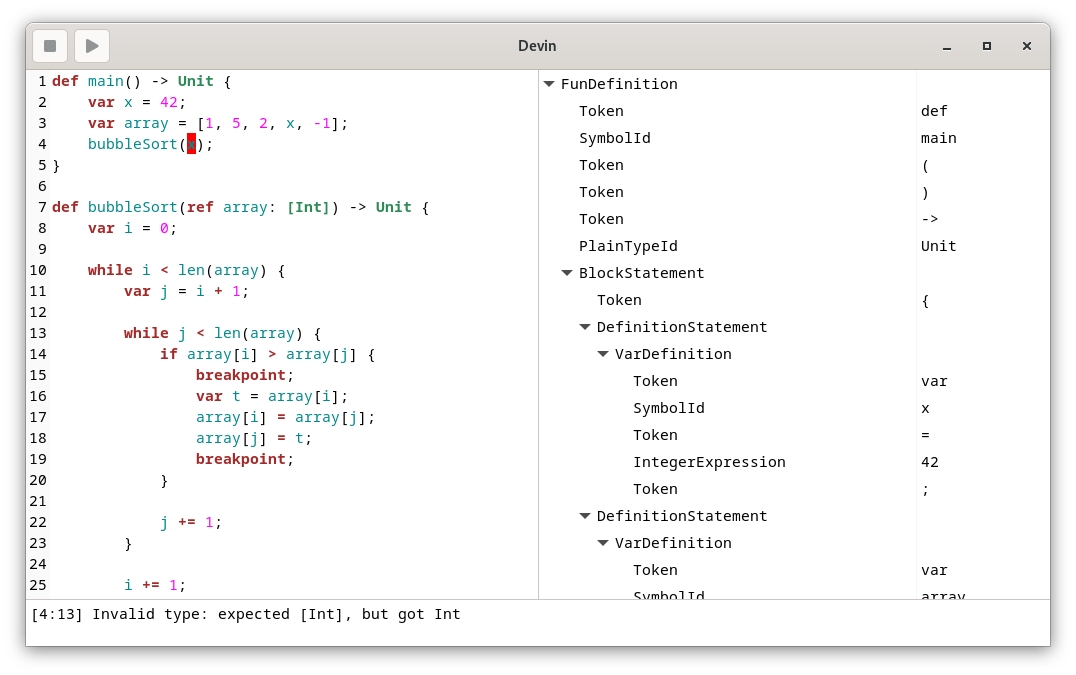
\includegraphics[width=0.9\linewidth]{4.png}
    \caption{Semantic error reporting and highlighting}
    \label{ex6}
  \end{figure}

  \begin{figure}[H]
    \center
    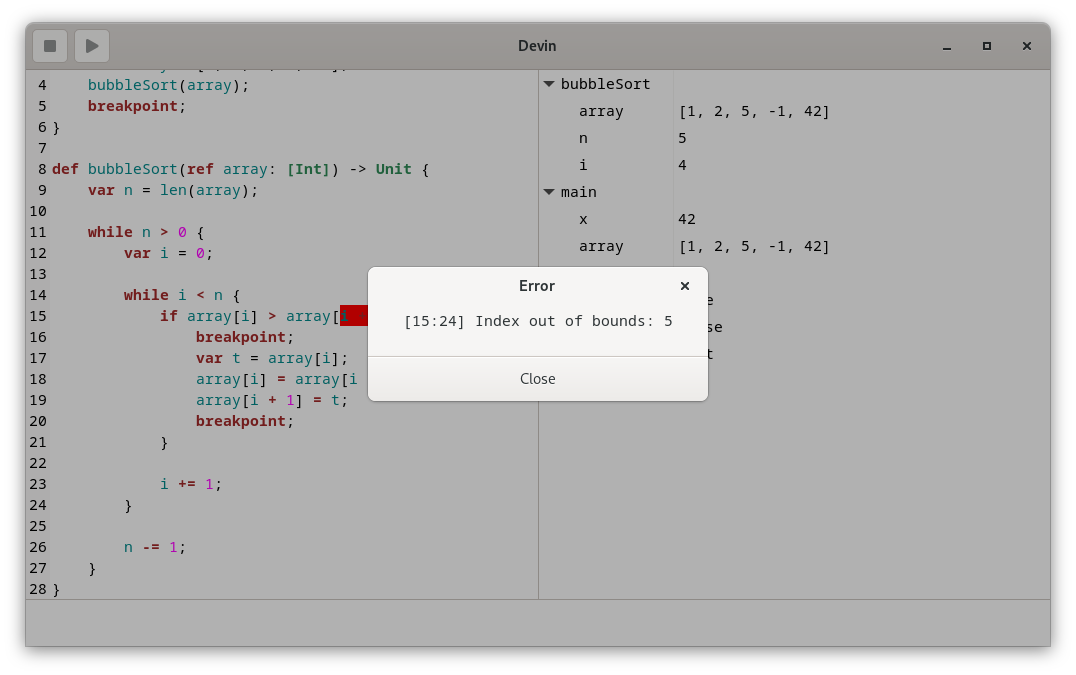
\includegraphics[width=0.9\linewidth]{6.png}
    \caption{Runtime error reporting and highlighting}
    \label{ex7}
  \end{figure}

  \begin{figure}[H]
    \center
    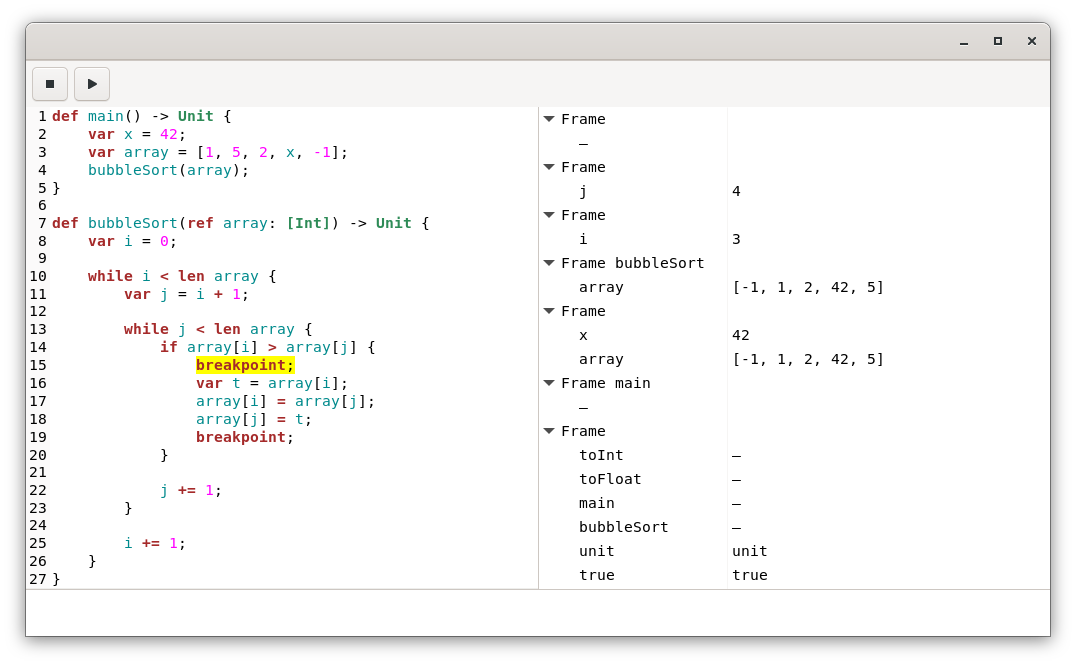
\includegraphics[width=0.9\linewidth]{5.png}
    \caption{The debugger}
    \label{ex8}
  \end{figure}


  \backmatter

  % \conclusions
  % TBD

  % \appendix

  % \chapter{Some technicalities}
  % TBD

  % \section{a section}
  % TBD

  \backmatter

  \bibliographystyle{plain}
  \bibliography{biblio}

  % \printindex  % use makeindex to generate the index
\end{document}
